%\setcounter{section}{2}
\section{Hàm số liên tục}
\subsection{Tóm tắt lý thuyết}
\begin{tomtat}
	\subsubsection{Hàm số liên tục tại một điểm}
	\begin{itemize}
		\item Cho hàm số $y=f(x)$ xác định trên khoảng $(a;b)$ chứa điểm $x_0$. Hàm số $f(x)$ được gọi là \textcolor{red}{liên tục tại điểm} $x_0$ nếu $\lim\limits_{x\to{x_0}}f(x)=f(x_0)$.
		\item Hàm số $f(x)$ không liên tục tại $x_0$ được gọi là \textcolor{red}{gián đoạn} tại điểm đó.
		\begin{note}
			Hàm số $y=f(x)$ liên tục tại $x_0$ khi và chỉ khi $\lim\limits_{x\to{x_0}^+}f(x)=\lim\limits_{x\to{x_0}^-}f(x)=f(x_0)$.
		\end{note}
	\end{itemize}
	\subsubsection{Hàm số liên tục trên một khoảng}
	\begin{itemize}
		\item Hàm số $y=f(x)$ được gọi là \textcolor{red}{liên tục trên khoảng} $(a;b)$ nếu nó liên tục tại mọi điểm thuộc khoảng này.
		\item Hàm số $y=f(x)$ được gọi là \textcolor{red}{liên tục trên đoạn} $[a;b]$ nếu nó liên tục trên khoảng $(a;b)$ và $\lim\limits_{x\to{a}^+}f(x)=f(a)$, $\lim\limits_{x\to{b}^-}f(x)=f(b)$.
		\item Các khái niệm hàm số liên tục trên nửa khoảng như $(a;b]$, $[a;+\infty)\ldots$ được định nghĩa theo cách tương tự.
		\item Đồ thị của hàm số liên tục trên một khoảng là một \textcolor{red}{đường liền nét} trên khoảng đó.
	\end{itemize}
	\subsubsection{Tính chất 1}
	\begin{itemize}
		\item Hàm số đa thức và các hàm số $y=\sin x$, $y=\cos x$ liên tục trên $\mathrm{R}$.
		\item Các hàm số $y=\tan x$, $y=\cot x$, $y=\sqrt x$ và các hàm phân thức hữu tỉ (thương của hai đa thức) liên tục trên mỗi khoảng xác định của chúng.
	\end{itemize}
	\subsubsection{Tính chất 2}
	Giả sử hai hàm số $y=f(x)$ và $y=g(x)$ liên tục tại điểm $x_0$. Khi đó:
	\begin{itemize}
		\item Các hàm số $y=f(x)+g(x)$, $y=f(x)-g(x)$ và $y=f(x)\cdot g(x)$ liên tục tại $x_0$.
		\item Hàm số $\dfrac{f(x)}{g(x)}$ liên tục tại $x_0$ nếu $g(x_0)\ne 0$.
	\end{itemize}
\end{tomtat}
\subsection{Các dạng toán thường gặp}
\begin{dang}{Dựa vào đồ thị xét tính liên tục của hàm số tại một điểm, một khoảng.}
		Để xét tính liên tục của hàm số khi biết đồ thị, ta cần nhớ:
	\begin{itemize}
		\item Đồ thị của hàm số liên tục trên một khoảng là một đường liền nét trên khoảng đó.
		\item Hàm số $y=f(x)$ liên tục tại $x_0$ khi và chỉ khi $\lim\limits_{x\to{x_0}^+}f(x)=\lim\limits_{x\to{x_0}^-}f(x)=f(x_0)$.
	\end{itemize}
\end{dang}
\subsubsection{Ví dụ mẫu}
\begin{vd}%[DCHT Toán 11 - KNTT -Vũ Hồng Toàn]%[1K5YG-2]
	\immini{
	Cho hàm số $y=f(x)$ có đồ thị như hình vẽ bên.\\ Xét tính liên tục của hàm số $y=f(x)$ trên khoảng $(0;2)$.	
	}
	{
	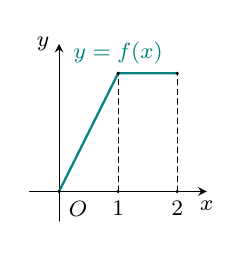
\begin{tikzpicture}[scale=.75, font=\footnotesize, line join=round, line cap=round,>=stealth]
		\def\xmin{-.5} \def\xmax{2.5}
		\def\ymin{-0.5} \def\ymax{2.5}
		\draw[->] (\xmin,0)--(0,0)node [below right]{$O$}-- (\xmax,0) node [below]{$x$};
		\draw[->] (0,\ymin)--(0,\ymax) node [left]{$y$};
		\draw[teal, thick] (0,0)--(1,2)--(2,2);
		\draw[dash pattern=on 2pt off 1.5pt] (1,0)node[below]{$1$}--(1,2) (2,0)node[below]{$2$}--(2,2)  (1,2)node[above,teal]{$y=f(x)$};
		\foreach \x/\y in{0/0,1/0,2/0,1/2,2/2} \fill(\x,\y)circle(.03);
	\end{tikzpicture}		
	}
	\dapso{Hàm số liên tục trên khoảng $(0;2)$.}
	\loigiai{
		Đồ thị hàm số là một đường liền nét trên khoảng $(0;2)$ nên hàm số đã cho liên tục trên khoảng $(0;2)$.}
\end{vd}
\begin{vd}%[DCHT Toán 11 - KNTT -Vũ Hồng Toàn]%[1K5YG-2]
	\immini{
	Cho hàm số $y=f(x)$ có đồ thị như hình vẽ bên.\\ Xét tính liên tục của hàm số $y=f(x)$ trên khoảng $(-2;2)$.	
	}
	{
	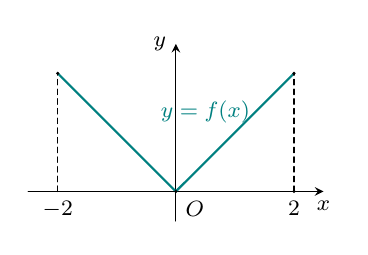
\begin{tikzpicture}[scale=.75, font=\footnotesize, line join=round, line cap=round,>=stealth]
		\def\xmin{-2.5} \def\xmax{2.5}
		\def\ymin{-0.5} \def\ymax{2.5}
		\draw[->] (\xmin,0)--(0,0)node [below right]{$O$}-- (\xmax,0) node [below]{$x$};
		\draw[->] (0,\ymin)--(0,\ymax) node [left]{$y$};
		\draw[teal, thick] plot[domain=-2:2](\x,{abs(\x)});
		\draw[dash pattern=on 2pt off 1.5pt] (-2,0)node[below]{$-2$}--(-2,2) (2,0)node[below]{$2$}--(2,2)  (.5,1)node[above,teal]{$y=f(x)$};
		\foreach \x/\y in{0/0,2/0,-2/2,2/2} \fill(\x,\y)circle(.03);
	\end{tikzpicture}		
	}
	\dapso{Hàm số liên tục trên khoảng $(-2;2)$.}
	\loigiai{
		Đồ thị hàm số là một đường liền nét trên khoảng $(-2;2)$ nên hàm số đã cho liên tục trên khoảng $(-2;2)$.}
\end{vd}

\begin{vd}%[DCHT Toán 11 - KNTT -Vũ Hồng Toàn]%[1K5BG-2]
	\immini{
	Cho hàm số $y=f(x)$ có đồ thị như hình vẽ bên.\\ Xét tính liên tục của hàm số $y=f(x)$ trên khoảng $(0;2)$.	
	}
	{
	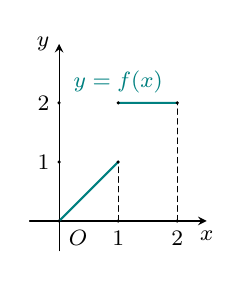
\begin{tikzpicture}[scale=.75, font=\footnotesize, line join=round, line cap=round,>=stealth]
		\def\xmin{-.5} \def\xmax{2.5}
		\def\ymin{-0.5} \def\ymax{3}
		\draw[->] (\xmin,0)--(0,0)node [below right]{$O$}-- (\xmax,0) node [below]{$x$};
		\draw[->] (0,\ymin)--(0,\ymax) node [left]{$y$};
		\draw[teal, thick] (0,0)--(1,1) (1,2)--(2,2);
		\draw[dash pattern=on 2pt off 1.5pt] (1,0)node[below]{$1$}--(1,1) (2,0)node[below]{$2$}--(2,2) (0,1)node[left]{$1$} (0,2)node[left]{$2$}
		(1,2)node[above,teal]{$y=f(x)$}
		;
		\foreach \x/\y in{0/0,1/0,2/0,1/2,2/2,1/1,0/1,0/2} \fill(\x,\y)circle(.03);
	\end{tikzpicture}		
	}
	
	\dapso{Hàm số đã cho liên tục trên các khoảng $(0,1)$, $(1,2)$ và gián đoạn tại $x=1$.}
	\loigiai{
		\begin{itemize}
			\item Đồ thị hàm số là các đường liền nét trên các khoảng $(0;1)$, $(1;2)$ do đó hàm số liên tục trên các khoảng này.
			\item Đồ thị hàm số không liền nét tại điểm $x=1$ do đó hàm số đã cho gián đoạn tại điểm này.
		\end{itemize}
	}
\end{vd}
\begin{vd}%[DCHT Toán 11 - KNTT -Vũ Hồng Toàn]%[1K5BG-2]
	\immini{
	Cho hàm số $y=f(x)$ có đồ thị như hình vẽ bên.\\ Xét tính liên tục của hàm số $y=f(x)$ trên khoảng $(0;2)$.	
	}
	{
	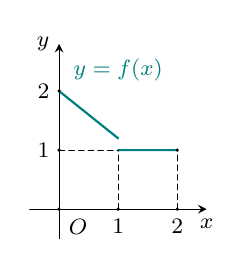
\begin{tikzpicture}[scale=.75, font=\footnotesize, line join=round, line cap=round,>=stealth]
		\def\xmin{-.5} \def\xmax{2.5}
		\def\ymin{-0.5} \def\ymax{2.8}
		\draw[->] (\xmin,0)--(0,0)node [below right]{$O$}-- (\xmax,0) node [below]{$x$};
		\draw[->] (0,\ymin)--(0,\ymax) node [left]{$y$} ;
		\draw[teal, thick] (1,1)--(2,1) (0,2)--(1,1.2);
		\draw[dash pattern=on 2pt off 1.5pt] (1,0)node[below]{$1$}--(1,1) (2,0)node[below]{$2$}--(2,1) (0,1)node[left]{$1$} (0,2)node[left]{$2$} (0,1)--(1,1)
		(1,2)node[above,teal]{$y=f(x)$}
		;
		\foreach \x/\y in{0/0,1/0,2/0,2/1,0/1,0/2} \fill(\x,\y)circle(.03);
	\end{tikzpicture}		
	}
	\dapso{Hàm số đã cho liên tục trên các khoảng $(0,1)$, $(1,2)$ và gián đoạn tại $x=1$.}
	\loigiai{
		\begin{itemize}
			\item Đồ thị hàm số là các đường liền nét trên các khoảng $(0;1)$, $(1;2)$ do đó hàm số liên tục trên các khoảng này.
			\item Ta có $\lim\limits_{x\to{1}^-}f(x)>f(1)=1$ và $\lim\limits_{x\to{1}^+}f(x)=f(1)=1$.\\ Do đó $\lim\limits_{x\to{1}^-}f(x)\ne \lim\limits_{x\to{1}^+}f(x)$.\\
			Vậy hàm số đã cho gián đoạn tại $x=1$.
		\end{itemize}
	}
\end{vd}

\begin{vd}%[DCHT Toán 11 - KNTT -Vũ Hồng Toàn]%[1K5KG-2]
	\immini{
	Cho hàm số $y=f(x)$ có tập xác định $\mathscr{D}=\mathbb{R}\setminus \{0\}$ và có đồ thị như hình bên. Xét tính liên tục của hàm số $y=f(x)$ trên $\mathscr{D}$.	
	}
	{
	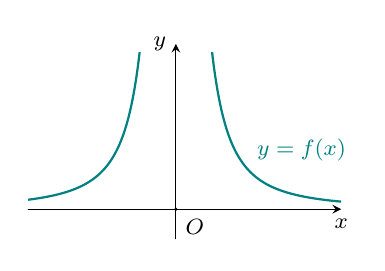
\begin{tikzpicture}[scale=.75, font=\footnotesize, line join=round, line cap=round,>=stealth]
		\def\xmin{-2.5} \def\xmax{2.8}
		\def\ymin{-0.5} \def\ymax{2.8}
		%\draw[color=gray!50,dashed] (\xmin,\ymin) grid (\xmax,\ymax);
		\draw[->] (\xmin,0)--(0,0)node [below right]{$O$}-- (\xmax,0) node [below]{$x$};
		\draw[->] (0,\ymin)--(0,\ymax) node [left]{$y$};
		\begin{scope}
			\clip (\xmin,\ymin) rectangle (\xmax,\ymax-.15);
			\draw[samples=200,smooth,variable=\x,thick, teal] plot[domain=\xmin:-0.5] (\x,{1/(\x)^2});
			\draw[samples=200,smooth,variable=\x,thick, teal] plot[domain=0.5:\xmax] (\x,{1/(\x)^2});
		\end{scope}
		\draw[teal, thick] (1.2,1)node[right]{$y=f(x)$};
		\foreach \x/\y in{0/0} \fill(\x,\y)circle(.03);
	\end{tikzpicture}	
	}
	\dapso{Hàm số đã cho liên tục trên các khoảng $(-\infty;0)$ và $(0;+\infty)$. Gián đoạn tại điểm $x=0$.}
	\loigiai{
	Vì hàm số đã cho có tập xác định $\mathscr{D}=\mathbb{R}\setminus \{0\}$ nên
	\begin{itemize}
		\item $f(x)$ xác định trên khoảng $(-\infty;0)$ nên liên tục trên khoảng này.
		\item $f(x)$ xác định trên khoảng $(0;+\infty)$ nên liên tục trên khoảng này.
		\item $f(x)$ không xác định tại điểm $x=0$ nên gián đoạn tại điểm này.
	\end{itemize}	
	}
\end{vd}

\subsubsection{Bài tập rèn luyện}
\centerline{\fcolorbox{teal}{yellow!50}{\bf {BÀI TẬP TỰ LUẬN }}}
\begin{bt}%[DCHT Toán 11 - KNTT -Vũ Hồng Toàn]%[1K5YG-2]
\immini[thm]{
Cho hàm số $y=f(x)$ xác định trên $\mathscr{D}=\mathbb{R}$ và có đồ thị như hình vẽ bên.\\ Xét tính liên tục của hàm số $y=f(x)$ trên $\mathscr{D}$.	
}
{
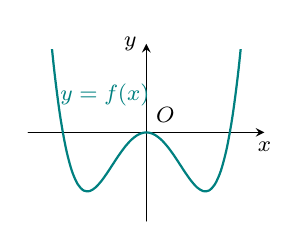
\begin{tikzpicture}[scale=.75, font=\footnotesize, line join=round, line cap=round,>=stealth]
	\def\a{1} \def\b{-2} \def\c{0} %\def\d{1} % Hệ số
	\def\xmin{-2} \def\xmax{2}
	\def\ymin{-1.5} \def\ymax{1.5}
	\draw[->] (\xmin,0)--(0,0)node [above right]{$O$}-- (\xmax,0) node [below]{$x$};
	\draw[->] (0,\ymin)--(0,\ymax) node [left]{$y$};
	\clip (\xmin+0.1,\ymin+0.1) rectangle (\xmax-0.1,\ymax-0.1);
	\draw[smooth,samples=100,thick,teal] plot(\x,{\a*(\x)^4+\b*(\x)^2+\c});
	\draw[teal, thick] (-.7,1)node[below]{$y=f(x)$};
\end{tikzpicture}	
}	
	\dapso{Hàm số đã cho liên tục trên $\mathbb{R}$.}
	\loigiai{
		Do đồ thị hàm số là một đường liền nét trên $\mathscr{D}$ nên hàm số $y=f(x)$ liên tục trên $\mathscr{D}=\mathbb{R}$.}
\end{bt}
\begin{bt}%[DCHT Toán 11 - KNTT -Vũ Hồng Toàn]%[1K5BG-2]
	\immini[thm]{
	Cho hàm số $y=f(x)$ xác định trên $\mathscr{D}=\mathbb{R}$ và có đồ thị như hình vẽ bên. Xét tính liên tục của hàm số $y=f(x)$ trên $\mathscr{D}$.	
	}
	{
	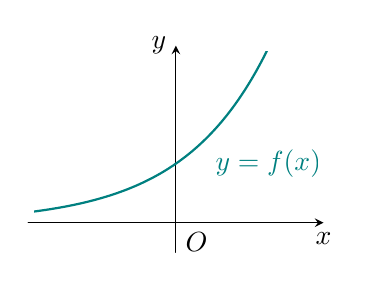
\begin{tikzpicture}[scale=.75, font=\normalsize, line join=round, line cap=round,>=stealth]
		\def\a{2} %\def\b{-2} \def\c{0} %\def\d{1} % Hệ số
		\def\xmin{-2.5} \def\xmax{2.5}
		\def\ymin{-0.5} \def\ymax{3}
		%\draw[color=gray!50,dashed] (\xmin,\ymin) grid (\xmax,\ymax);
		\draw[->] (\xmin,0)--(0,0)node [below right]{$O$}-- (\xmax,0) node [below]{$x$};
		\draw[->] (0,\ymin)--(0,\ymax) node [left]{$y$};
		\clip (\xmin+0.1,\ymin+0.1) rectangle (\xmax-0.1,\ymax-0.1);
		\draw[smooth,samples=100,thick,teal] plot(\x,{\a^(\x)}) (.5,1) node [right]{$y=f(x)$};
	\end{tikzpicture}	
	}
	\dapso{Hàm số đã cho liên tục trên $\mathbb{R}$.}
	\loigiai{
		Do đồ thị hàm số là một đường liền nét trên $\mathscr{D}$ nên hàm số $y=f(x)$ liên tục trên $\mathscr{D}=\mathbb{R}$.}
\end{bt}
\begin{bt}%[DCHT Toán 11 - KNTT -Vũ Hồng Toàn]%[1K5KG-2]
	\immini[thm]{
	Cho hàm số $y=f(x)$ xác định trên $\mathscr{D}=\mathbb{R}$ và có đồ thị như hình vẽ bên. Xét tính liên tục của hàm số $y=f(x)$ trên $\mathscr{D}$.	
	}
	{
	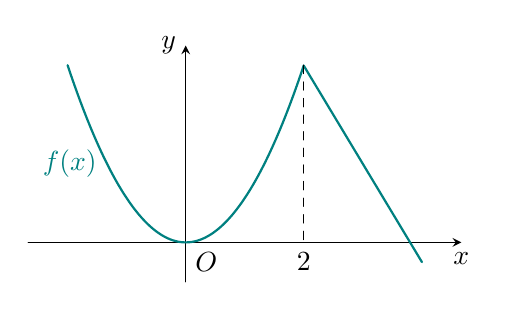
\begin{tikzpicture}[scale=1, font=\normalsize, line join=round, line cap=round,>=stealth]
		\def\xmin{-2} \def\xmax{3.5}
		\def\ymin{-.5} \def\ymax{2.5}
		\draw[->] (\xmin,0)--(0,0)node [below right]{$O$}-- (\xmax,0) node [below]{$x$};
		\draw[->] (0,\ymin)--(0,\ymax) node [left]{$y$};
		\clip (\xmin+0.1,\ymin+0.1) rectangle (\xmax-0.1,\ymax-0.1);
		\draw[smooth,samples=100,thick,teal] plot[domain=-1.5:1.5](\x,{(\x)^2})--(3,-.25) 
		(-1,1) node [left]{$y=f(x)$}; 
		\draw[dashed] (1.5,2.25)--(1.5,0) node [below]{$2$} ;
	\end{tikzpicture}	
	}
	
	\dapso{Hàm số đã cho liên tục trên $\mathbb{R}$.}
	\loigiai{
		Do đồ thị hàm số là một đường liền nét trên $\mathscr{D}$ nên hàm số $y=f(x)$ liên tục trên $\mathscr{D}=\mathbb{R}$.}
\end{bt}
\begin{bt}%[DCHT Toán 11 - KNTT -Vũ Hồng Toàn]%[1K5KG-2]
	\immini[thm]{
	Cho hàm số $y=f(x)$ có đồ thị như hình vẽ bên.\\ Xét tính liên tục của hàm số $y=f(x)$ tại điểm $x_0=2$.	
	}
	{
	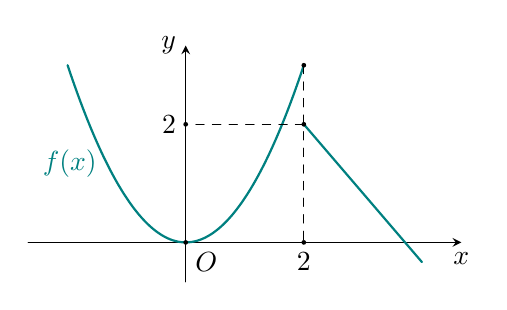
\begin{tikzpicture}[scale=1, font=\normalsize, line join=round, line cap=round,>=stealth]
		\def\xmin{-2} \def\xmax{3.5}
		\def\ymin{-.5} \def\ymax{2.5}
		\draw[->] (\xmin,0)--(0,0)node [below right]{$O$}-- (\xmax,0) node [below]{$x$};
		\draw[->] (0,\ymin)--(0,\ymax) node [left]{$y$};
		\clip (\xmin+0.1,\ymin+0.1) rectangle (\xmax-0.1,\ymax-0.1);
		\draw[smooth,samples=100,thick,teal] plot[domain=-1.5:1.5](\x,{(\x)^2}) (1.5,1.5)--(3,-.25) 
		(-1,1) node [left]{$y=f(x)$}; 
		\draw[dashed] (1.5,2.25)--(1.5,0) node [below]{$2$} (1.5,1.5)--(0,1.5)node [left]{$2$};
		\foreach \x/\y in{0/0,1.5/0,1.5/1.5,0/1.5,1.5/2.25} \fill(\x,\y)circle(.03);
	\end{tikzpicture}	
	}
	\dapso{Hàm số đã cho gián đoạn tại $x_0=2$. }
	\loigiai{
		Ta có $\lim\limits_{x\to{2}^-}f(x)>2$ và $\lim\limits_{x\to{2}^+}f(x)=2$. Do đó $\lim\limits_{x\to{2}^-}f(x)\ne \lim\limits_{x\to{2}^+}f(x)$. Vậy hàm số đã cho gián đoạn tại $x_0=2$.
	}
\end{bt}

\begin{bt}%[DCHT Toán 11 - KNTT -Vũ Hồng Toàn]%[1K5KG-2]
	\immini[thm]{
	Cho hàm số $y=f(x)$ có đồ thị như hình vẽ bên.\\ Xét tính liên tục của hàm số $y=f(x)$ tại điểm $x_0=1$.	
	}
	{
	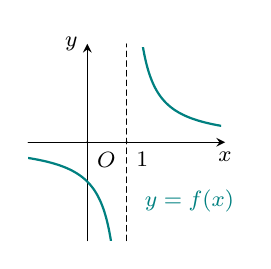
\begin{tikzpicture}[scale=.5, font=\footnotesize, line join=round, line cap=round,>=stealth]
		\def\a{0} \def\b{1} \def\c{1} \def\d{-1}
		\pgfmathsetmacro\tcd{int(round(-\d/\c))} \pgfmathsetmacro\tcn{int(round(\a/\c))} 
		\pgfmathsetmacro\xmin{\tcd-2.5} \pgfmathsetmacro\xmax{\tcd+2.5}
		\pgfmathsetmacro\ymin{\tcn-2.5} \pgfmathsetmacro\ymax{\tcn+2.5}
		\draw[->] (\xmin,0)--(0,0)node [below right]{$O$}-- (\xmax,0) node [below]{$x$};
		\draw[->] (0,\ymin)--(0,\ymax) node [left]{$y$};
		\draw[dash pattern=on 2pt off 1.5pt] (\tcd,\ymin)--(\tcd,\ymax) (\tcd,0)node [below right]{$\tcd$};
		\begin{scope}
			\clip (\xmin,\ymin) rectangle (\xmax-.1,\ymax-.1);
			\draw[samples=200,smooth,variable=\x,thick, teal] plot[domain=\xmin:\tcd-0.3] (\x,{(\a*(\x)+\b)/(\c*(\x)+\d)});
			\draw[samples=200,smooth,variable=\x,thick, teal] plot[domain=\tcd+.3:\xmax] (\x,{(\a*(\x)+\b)/(\c*(\x)+\d)});
		\end{scope}
		\draw[teal, thick] (1.2,-1.5)node[right]{$y=f(x)$};
		\foreach \x/\y in{0/0,1/0} \fill(\x,\y)circle(.03);
	\end{tikzpicture}	
	}
	\dapso{Hàm số đã cho gián đoạn tại $x_0=1$. }
	\loigiai{
		Ta có $\lim\limits_{x\to{1}^-}f(x)=-\infty$ và $\lim\limits_{x\to{1}^+}f(x)=+\infty$. Do đó $\lim\limits_{x\to{1}^-}f(x)\ne \lim\limits_{x\to{1}^+}f(x)$.\\ Vậy hàm số đã cho gián đoạn tại $x_0=1$.
	}
\end{bt}

\centerline{\fcolorbox{teal}{yellow!50}{\bf {CÂU HỎI TRẮC NGHIỆM (10 câu theo theo tỉ lệ 4:3:2:1)}}}
\Opensolutionfile{ans}[ans/ans-1K5-3-Dang1]

\begin{ex}%[DCHT Toán 11 - KNTT -Vũ Hồng Toàn]%[1K5YG-2]
\immini[thm]{
Cho đồ thị hàm số $y=f(x)$ có đồ thị như hình vẽ bên. Chọn mệnh đề đúng trong các mệnh đề sau:
\choice[1]
{Hàm số $y=f(x)$ liên tục trên $\mathbb{R}$}
{\True Hàm số $y=f(x)$ liên tục trên khoảng $(0,+\infty)$}
{Hàm số $y=f(x)$ liên tục tại điểm $x_0=0$}
{$\lim\limits_{x\to{0}^+}f(x)=+\infty$}	
}
{
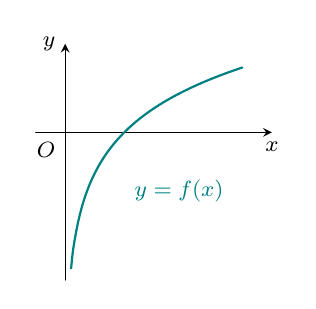
\begin{tikzpicture}[scale=.75, font=\footnotesize, line join=round, line cap=round,>=stealth]
	\def\xmin{-.5} \def\xmax{3.5}
	\def\ymin{-2.5} \def\ymax{1.5}
	\draw[->] (\xmin,0)--(0,0)node [below left]{$O$}-- (\xmax,0) node [below]{$x$};
	\draw[->] (0,\ymin)--(0,\ymax) node [left]{$y$};
	\clip (\xmin+0.1,\ymin+0.1) rectangle (\xmax-0.1,\ymax-0.1);
	\draw[smooth,samples=100,thick,teal] plot[domain=.1:3](\x,{ln(\x)}) 
	(1,-1) node [right]{$y=f(x)$}; 
\end{tikzpicture}	
}	
	\loigiai
	{
	Đồ thị hàm số là một đường liền nét trên khoảng $(0,+\infty)$ nên liên tục trên khoảng này.
	}
\end{ex}
%Cau2
\begin{ex}%[DCHT Toán 11 - KNTT -Vũ Hồng Toàn]%[1K5YG-2]
\immini[thm]{
Cho đồ thị hàm số $y=f(x)$ có đồ thị như hình vẽ bên. Chọn mệnh đề \textbf{sai} trong các mệnh đề sau:
\choice[1]
{\True $\lim\limits_{x\to{+\infty}}f(x)=-\infty$}
{Hàm số $y=f(x)$ liên tục trên $\mathbb{R}$}
{$\lim\limits_{x\to{+\infty}}f(x)=+\infty$}
{$\lim\limits_{x\to{-\infty}}f(x)=-\infty$}	
}
{
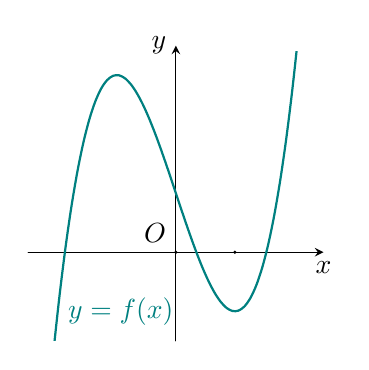
\begin{tikzpicture}[scale=.75, font=\normalsize, line join=round, line cap=round,>=stealth]
	\def\a{1} \def\b{0} \def\c{-3} \def\d{1}
	\def\f(#1){\a*(#1)^3+\b*(#1)^2+\c*(#1)+\d}
	\pgfmathsetmacro\tdx{int(round(-\b/(3*\a)))} \pgfmathsetmacro\tdy{int(round(\f(\tdx))}
	\pgfmathsetmacro\xmin{\tdx-2.5} \pgfmathsetmacro\xmax{\tdx+2.5}
	\pgfmathsetmacro\ymin{\tdy-2.5} \pgfmathsetmacro\ymax{\tdy+2.5}
	%\draw[color=gray!50,dashed] (\xmin,\ymin) grid (\xmax,\ymax);
	\draw[->] (\xmin,0)--(0,0)node [above left]{$O$}-- (\xmax,0) node [below]{$x$};
	\draw[->] (0,\ymin)--(0,\ymax) node [left]{$y$};
	\begin{scope}
		\clip (\xmin,\ymin) rectangle (\xmax-.1,\ymax-.1);
		\draw[samples=100,smooth,thick, teal] plot(\x,{\f(\x)});
	\end{scope}
	\draw[teal, thick] (-2,-1)node[right]{$y=f(x)$};
	\foreach \x/\y in{0/0,1/0} \fill(\x,\y)circle(.03);
\end{tikzpicture} 	
}
	\loigiai
	{
	Quan sát đồ thị hàm số, ta có
	\begin{itemize}
		\item Hàm số $y=f(x)$ liên tục trên $\mathbb{R}$.
		\item $\lim\limits_{x\to{+\infty}}f(x)=+\infty$.
		\item $\lim\limits_{x\to{-\infty}}f(x)=-\infty$.
	\end{itemize}
	}
\end{ex}
%Cau3
\begin{ex}%[DCHT Toán 11 - KNTT -Vũ Hồng Toàn]%[1K5YG-2]
	\immini[thm]{
	Cho đồ thị hàm số $y=f(x)$ có đồ thị như hình vẽ bên. Chọn mệnh đề đúng trong các mệnh đề sau:
	\choice
	{$\lim\limits_{x\to{+\infty}}f(x)=-\infty$}
	{\True Hàm số $y=f(x)$ liên tục trên khoảng $(0;+\infty)$}
	{Hàm số $y=f(x)$ liên tục tại điểm $x_0=0$}
	{Hàm số $y=f(x)$ liên tục trên $\mathbb{R}$}	
	}
	{
	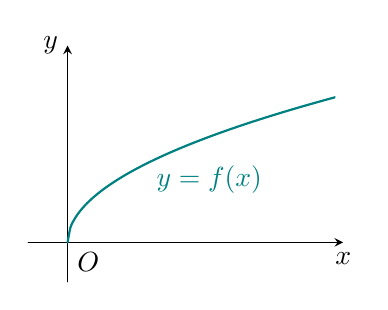
\begin{tikzpicture}[scale=1, font=\normalsize, line join=round, line cap=round,>=stealth]
		\def\xmin{-.5} \def\xmax{3.5}
		\def\ymin{-.5} \def\ymax{2.5}
		%\draw[color=gray!50,dashed] (\xmin,\ymin) grid (\xmax,\ymax);
		\draw[->] (\xmin,0)--(0,0)node [below right]{$O$}-- (\xmax,0) node [below]{$x$};
		\draw[->] (0,\ymin)--(0,\ymax) node [left]{$y$};
		\clip (\xmin+0.1,\ymin+0.1) rectangle (\xmax-0.1,\ymax-0.1);
		\draw[smooth,samples=100,thick,teal] plot[domain=0:3.5](\x,{sqrt(\x)}) 
		(1,.8) node [right]{$y=f(x)$}; 
	\end{tikzpicture}	
	}
	\loigiai
	{
	Quan sát đồ thị hàm số, thấy đồ thị hàm số là một đường liền nét trên khoảng $(0;+\infty)$ do đó hàm số đã cho liên tục trên khoảng này.
	}
\end{ex}
%Cau4
\begin{ex}%[DCHT Toán 11 - KNTT -Vũ Hồng Toàn]%[1K5YG-2]
	\immini[thm]{
	Cho đồ thị hàm số $y=f(x)$ có đồ thị như hình vẽ bên. Chọn mệnh đề \textbf{sai} trong các mệnh đề sau:
	\choice[1]
	{Hàm số gián đoạn tại điểm $x_0=0$}
	{Hàm số liên tục trên khoảng $(-\infty;0)$}
	{\True Hàm số $y=f(x)$ liên tục trên $\mathbb{R}$}
	{Hàm số liên tục trên khoảng $(0;+\infty)$}	
	}
	{
	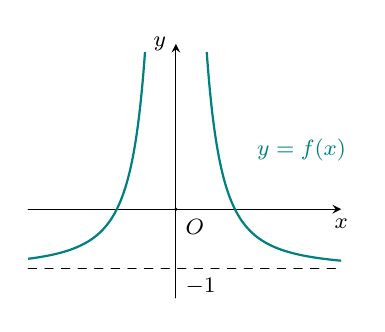
\begin{tikzpicture}[scale=.75, font=\footnotesize, line join=round, line cap=round,>=stealth]
		\def\xmin{-2.5} \def\xmax{2.8}
		\def\ymin{-1.5} \def\ymax{2.8}
		%\draw[color=gray!50,dashed] (\xmin,\ymin) grid (\xmax,\ymax);
		\draw[->] (\xmin,0)--(0,0)node [below right]{$O$}-- (\xmax,0) node [below]{$x$};
		\draw[->] (0,\ymin)--(0,\ymax) node [left]{$y$};
		\begin{scope}
			\clip (\xmin,\ymin) rectangle (\xmax,\ymax-.15);
			\draw[samples=200,smooth,variable=\x,thick, teal] plot[domain=\xmin:-0.5] (\x,{1/(\x)^2-1});
			\draw[samples=200,smooth,variable=\x,thick, teal] plot[domain=0.5:\xmax] (\x,{1/(\x)^2-1});
		\end{scope}
		\draw[dashed](\xmin,-1)--(\xmax,-1) (0,-1)node[below right]{$-1$};
		\draw[teal, thick] (1.2,1)node[right]{$y=f(x)$};
		\foreach \x/\y in{0/0} \fill(\x,\y)circle(.03);
	\end{tikzpicture}	
	}
	
	\loigiai
	{
		Quan sát đồ thị hàm số, ta có
		\begin{itemize}
			\item Hàm số gián đoạn tại điểm $x_0=0$.
			\item Hàm số liên tục trên khoảng $(-\infty;0)$.
			\item Hàm số liên tục trên khoảng $(0;+\infty)$.
		\end{itemize}
	}
\end{ex}
%Cau5
\begin{ex}%[DCHT Toán 11 - KNTT -Vũ Hồng Toàn]%[1K5BG-2]
\immini[thm]{
Cho đồ thị hàm số $y=f(x)$ có đồ thị như hình vẽ bên. Chọn mệnh đề \textbf{sai} trong các mệnh đề sau:
\choice[1]
{Hàm số gián đoạn tại điểm $x_0=1$}
{Hàm số liên tục trên khoảng $(-\infty;1)$}
{\True Hàm số $y=f(x)$ liên tục trên $\mathbb{R}$}
{Hàm số liên tục trên khoảng $(1;+\infty)$}		
}
{
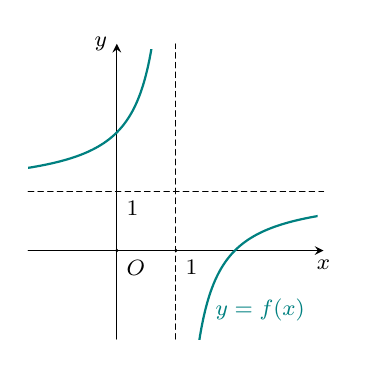
\begin{tikzpicture}[scale=.75, font=\footnotesize, line join=round, line cap=round,>=stealth]
	\def\a{1} \def\b{-2} \def\c{1} \def\d{-1}
	\pgfmathsetmacro\tcd{int(round(-\d/\c))} \pgfmathsetmacro\tcn{int(round(\a/\c))} 
	\pgfmathsetmacro\xmin{\tcd-2.5} \pgfmathsetmacro\xmax{\tcd+2.5}
	\pgfmathsetmacro\ymin{\tcn-2.5} \pgfmathsetmacro\ymax{\tcn+2.5}
	%\draw[color=gray!50,dashed] (\xmin,\ymin) grid (\xmax,\ymax);
	\draw[->] (\xmin,0)--(0,0)node [below right]{$O$}-- (\xmax,0) node [below]{$x$};
	\draw[->] (0,\ymin)--(0,\ymax) node [left]{$y$};
	\draw[dash pattern=on 2pt off 1.5pt] (\tcd,\ymin)--(\tcd,\ymax) (\tcd,0)node [below right]{$\tcd$}
	(\xmin,\tcn)--(\xmax,\tcn) (0,\tcn)node [below right]{$\tcn$};
	\begin{scope}
		\clip (\xmin,\ymin) rectangle (\xmax-.1,\ymax-.1);
		\draw[samples=200,smooth,variable=\x,thick, teal] plot[domain=\xmin:\tcd-0.3] (\x,{(\a*(\x)+\b)/(\c*(\x)+\d)});
		\draw[samples=200,smooth,variable=\x,thick, teal] plot[domain=\tcd+.3:\xmax] (\x,{(\a*(\x)+\b)/(\c*(\x)+\d)});
	\end{scope}
	\draw[teal, thick] (1.5,-1)node[right]{$y=f(x)$};
	\foreach \x/\y in{0/0,1/0} \fill(\x,\y)circle(.03);
\end{tikzpicture}	
}
	\loigiai
	{
		Quan sát đồ thị hàm số, ta có
		\begin{itemize}
			\item Hàm số gián đoạn tại điểm $x_0=1$.
			\item Hàm số liên tục trên khoảng $(-\infty;1)$.
			\item Hàm số liên tục trên khoảng $(1;+\infty)$.
		\end{itemize}
	}
\end{ex}
%Cau6
\begin{ex}%[DCHT Toán 11 - KNTT -Vũ Hồng Toàn]%[1K5BG-2]
	\immini{
	Cho đồ thị hàm số $y=f(x)$ có đồ thị như hình vẽ bên. Chọn mệnh đề đúng trong các mệnh đề sau:
	\choice[1]
	{Hàm số $y=f(x)$ liên tục trên $\mathbb{R}$}
	{$\lim\limits_{x\to{+\infty}}f(x)=-\infty$}
	{Hàm số liên tục tại điểm $x_0=-2$}
	{\True Hàm số gián đoạn tại điểm $x_0=-2$}	
	}
	{
	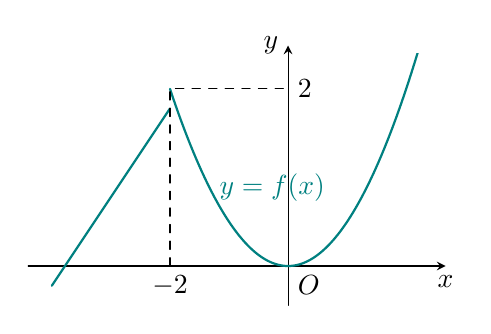
\begin{tikzpicture}[scale=1, font=\normalsize, line join=round, line cap=round,>=stealth]
		\def\xmin{-3.3} \def\xmax{2}
		\def\ymin{-.5} \def\ymax{2.8}
		\draw[->] (\xmin,0)--(0,0)node [below right]{$O$}-- (\xmax,0) node [below]{$x$};
		\draw[->] (0,\ymin)--(0,\ymax) node [left]{$y$} ;
		\clip (\xmin+0.1,\ymin+0.1) rectangle (\xmax-0.1,\ymax-0.1);
		\draw[smooth,samples=100,thick,teal] plot[domain=-1.5:2](\x,{(\x)^2})  
		(-1,1) node [right]{$y=f(x)$}; 
		\draw[thick,teal] (-3,-.25)--(-1.5,2);
		\draw[dashed] (-1.5,0)node [below]{$-2$}|-(0,2.25) node [right]{$2$} ;
	\end{tikzpicture}	
	} 
	 
	\loigiai
	{
	Quan sát đồ thị hàm số, ta có	
		\begin{itemize}
			\item Đồ thị hàm số là các đường liền nét trên các khoảng $(-\infty;-2)$, $(-2;+\infty)$ do đó hàm số liên tục trên các khoảng này.
			\item $\lim\limits_{x\to{+\infty}}f(x)=+\infty$
			\item Ta có $\lim\limits_{x\to{(-2)}^-}f(x)<f(-2)=2$ và $\lim\limits_{x\to{(-2)}^+}f(x)=f(-2)=2$. Do đó $\lim\limits_{x\to{(-2)}^-}f(x)\ne \lim\limits_{x\to{(-2)}^+}f(x)$.\\
			Vậy hàm số đã cho gián đoạn tại $x_0=-2$.
		\end{itemize}
	}
\end{ex}
%Cau7
\begin{ex}%[DCHT Toán 11 - KNTT -Vũ Hồng Toàn]%[1K5BG-2]
	 \immini[thm]{
	 Cho đồ thị hàm số $y=f(x)$ có đồ thị như hình vẽ bên. Chọn mệnh đề đúng trong các mệnh đề sau:
	 \choice[1]
	 {\True $\lim\limits_{x\to{1}^+}f(x)=+\infty$}
	 {Hàm số $y=f(x)$ liên tục trên $\mathbb{R}$}
	 {$\lim\limits_{x\to{1}^+}f(x)=-\infty$}
	 {$\lim\limits_{x\to{1}^-}f(x)=+\infty$}	
	 }
	 {
	 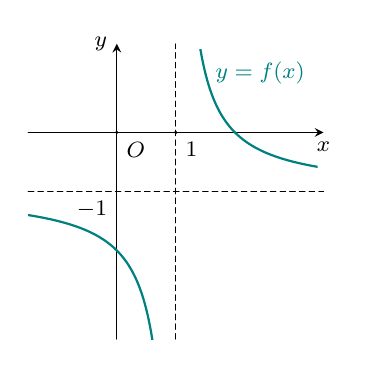
\begin{tikzpicture}[scale=.75, font=\footnotesize, line join=round, line cap=round,>=stealth]
	 	\def\a{-1} \def\b{2} \def\c{1} \def\d{-1}
	 	\pgfmathsetmacro\tcd{int(round(-\d/\c))} \pgfmathsetmacro\tcn{int(round(\a/\c))} 
	 	\pgfmathsetmacro\xmin{\tcd-2.5} \pgfmathsetmacro\xmax{\tcd+2.5}
	 	\pgfmathsetmacro\ymin{\tcn-2.5} \pgfmathsetmacro\ymax{\tcn+2.5}
	 	%\draw[color=gray!50,dashed] (\xmin,\ymin) grid (\xmax,\ymax);
	 	\draw[->] (\xmin,0)--(0,0)node [below right]{$O$}-- (\xmax,0) node [below]{$x$};
	 	\draw[->] (0,\ymin)--(0,\ymax) node [left]{$y$};
	 	\draw[dash pattern=on 2pt off 1.5pt] (\tcd,\ymin)--(\tcd,\ymax) (\tcd,0)node [below right]{$\tcd$}
	 	(\xmin,\tcn)--(\xmax,\tcn) (0,\tcn)node [below left]{$\tcn$};
	 	\begin{scope}
	 		\clip (\xmin,\ymin) rectangle (\xmax-.1,\ymax-.1);
	 		\draw[samples=200,smooth,variable=\x,thick, teal] plot[domain=\xmin:\tcd-0.3] (\x,{(\a*(\x)+\b)/(\c*(\x)+\d)});
	 		\draw[samples=200,smooth,variable=\x,thick, teal] plot[domain=\tcd+.3:\xmax] (\x,{(\a*(\x)+\b)/(\c*(\x)+\d)});
	 	\end{scope}
	 	\draw[teal, thick] (1.5,1)node[right]{$y=f(x)$};
	 	\foreach \x/\y in{0/0,1/0} \fill(\x,\y)circle(.03);
	 \end{tikzpicture}	
	 }
	 
	\loigiai
	{
		Quan sát đồ thị hàm số, ta có	
		\begin{itemize}
			\item Đồ thị hàm số là các đường liền nét trên các khoảng $(-\infty;1)$, $(1;+\infty)$ do đó hàm số liên tục trên các khoảng này.
			\item $\lim\limits_{x\to{+\infty}}f(x)=-1$.
			\item Ta có $\lim\limits_{x\to{1}^-}f(x)=-\infty$ và $\lim\limits_{x\to{1}^+}f(x)=+\infty$. Do đó $\lim\limits_{x\to{1}^-}f(x)\ne \lim\limits_{x\to{1}^+}f(x)$.\\
			Vậy hàm số đã cho gián đoạn tại $x_0=1$.
		\end{itemize}
	}
\end{ex}
%Cau8
\begin{ex}%[DCHT Toán 11 - KNTT -Vũ Hồng Toàn]%[1K5KG-2]
	\immini[thm]{
	Cho đồ thị hàm số $y=f(x)$ có đồ thị như hình vẽ bên. Chọn mệnh đề đúng trong các mệnh đề sau:
	\choice[1]
	{Hàm số $y=f(x)$ gián đoạn tại $x_0=0$}
	{$\lim\limits_{x\to{+\infty}}f(x)=-1$}
	{$\lim\limits_{x\to{-\infty}}f(x)=-1$}
	{\True Hàm số $y=f(x)$ liên tục trên $\mathbb{R}$}	
	}
	{
	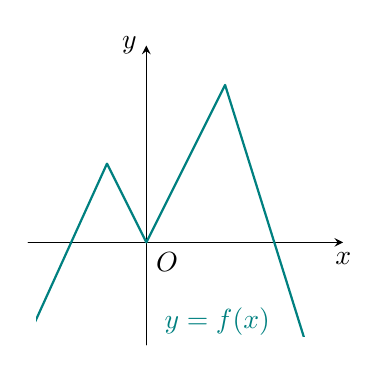
\begin{tikzpicture}[scale=1, font=\normalsize, line join=round, line cap=round,>=stealth]
		%	\def\a{2} %\def\b{-2} \def\c{0} %\def\d{1} % Hệ số
		\def\xmin{-1.5} \def\xmax{2.5}
		\def\ymin{-1.3} \def\ymax{2.5}
		%\draw[color=gray!50,dashed] (\xmin,\ymin) grid (\xmax,\ymax);
		\draw[->] (\xmin,0)--(0,0)node [below right]{$O$}-- (\xmax,0) node [below]{$x$};
		\draw[->] (0,\ymin)--(0,\ymax) node [left]{$y$};
		\clip (\xmin+0.1,\ymin+0.1) rectangle (\xmax-0.1,\ymax-0.1);
		\draw[thick,teal] (-1.5,-1.2)--(-.5,1)--(0,0)--(1,2)--(2,-1.2) 
		(1.7,-1) node [left]{$y=f(x)$}; 
	\end{tikzpicture}	
	}
	 
	\loigiai
	{
		Quan sát đồ thị hàm số, ta có	
		\begin{itemize}
			\item Đồ thị hàm số là các đường liền nét trên khoảng $(-\infty;+\infty)$ do đó hàm số liên tục trên $\mathbb{R}$.
			\item $\lim\limits_{x\to{+\infty}}f(x)=-\infty$.
			\item $\lim\limits_{x\to{-\infty}}f(x)=-\infty$.
		\end{itemize}
	}
\end{ex}
%Cau9
\begin{ex}%[DCHT Toán 11 - KNTT -Vũ Hồng Toàn]%[1K5KG-2]
	 \immini[thm]{
	 Cho đồ thị hàm số $y=f(x)$ có đồ thị như hình vẽ bên. Chọn mệnh đề đúng trong các mệnh đề sau:
	 \choice[1]
	 {Hàm số $y=f(x)$ liên tục trên $\mathbb{R}$}
	 {Hàm số $y=f(x)$ liên tục tại $x_0=-3$}
	 {$\lim\limits_{x\to{-\infty}}f(x)=-\infty$}
	 {\True Hàm số $y=f(x)$ gián đoạn tại $x_0=3$}	
	 }
	 {
	 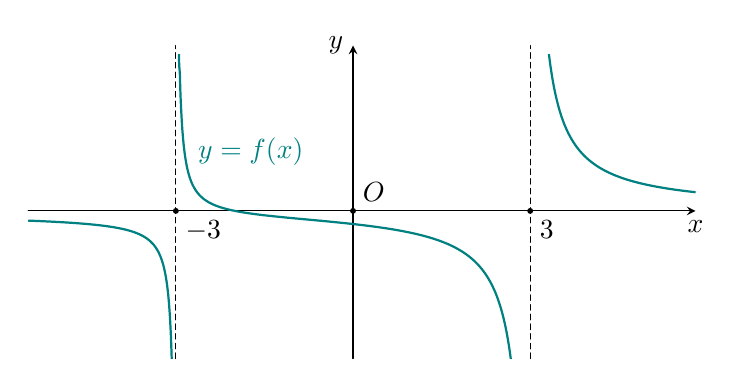
\begin{tikzpicture}[scale=.75, font=\normalsize, line join=round, line cap=round,>=stealth]
	 	\def\xmin{-5.5} \def\xmax{5.8}
	 	\def\ymin{-2.5} \def\ymax{2.8}
	 	%\draw[color=gray!50,dashed] (\xmin,\ymin) grid (\xmax,\ymax);
	 	\draw[->] (\xmin,0)--(0,0)node [above right]{$O$}-- (\xmax,0) node [below]{$x$};
	 	\draw[->] (0,\ymin)--(0,\ymax) node [left]{$y$};
	 	\draw[dash pattern=on 2pt off 1.5pt] (-3,\ymin)--(-3,\ymax) (3,\ymin)--(3,\ymax)
	 	(-3,0)node [below right]{$-3$} (3,0)node [below right]{$3$}
	 	;
	 	\begin{scope}
	 		\clip (\xmin,\ymin) rectangle (\xmax,\ymax-.15);
	 		\draw[samples=200,smooth,variable=\x,thick, teal] plot[domain=\xmin:-3.01] (\x,{(\x+2)/((\x)^2-9)});
	 		\draw[samples=200,smooth,variable=\x,thick, teal] plot[domain=-2.99:2.99] (\x,{(\x+2)/((\x)^2-9)});
	 		\draw[samples=200,smooth,variable=\x,thick, teal] plot[domain=3.01:\xmax] (\x,{(\x+2)/((\x)^2-9)});
	 	\end{scope}
	 	\draw[teal, thick] (-2.8,1)node[right]{$y=f(x)$};
	 	\foreach \x/\y in{0/0,-3/0,3/0} \fill(\x,\y)circle(.05);
	 \end{tikzpicture} 	
	 }
	\loigiai
	{
		Quan sát đồ thị hàm số, ta có	
		\begin{itemize}
			\item Đồ thị hàm số là các đường liền nét trên khoảng $(-\infty;-3)$, $(-3;3)$, $(3;+\infty) $ do đó hàm số liên tục trên các khoảng này.
			\item $\lim\limits_{x\to{-\infty}}f(x)=0$.
			\item Hàm số $y=f(x)$ gián đoạn tại các điểm $x_0=3$ và $x_0=-3$.
		\end{itemize}
	}
\end{ex}
%Cau10
\begin{ex}%[DCHT Toán 11 - KNTT -Vũ Hồng Toàn]%[1K5GG-2]
	 \immini[thm]{
	 Cho đồ thị hàm số $y=f(x)$ có đồ thị như hình vẽ bên. Chọn mệnh đề đúng trong các mệnh đề sau:
	 \choice[1]
	 {Hàm số $y=f(x)$ liên tục trên $\mathbb{R}$}
	 {Hàm số $y=f(x)$ liên tục tại điểm $x_0=\dfrac{\pi}{2}$}
	 {Hàm số $y=f(x)$ liên tục tại điểm $x_0=-\dfrac{\pi}{2}$}
	 {\True Hàm số $y=f(x)$ gián đoạn tại điểm $x_0=\dfrac{\pi}{2}$}
	 }
	 {
	 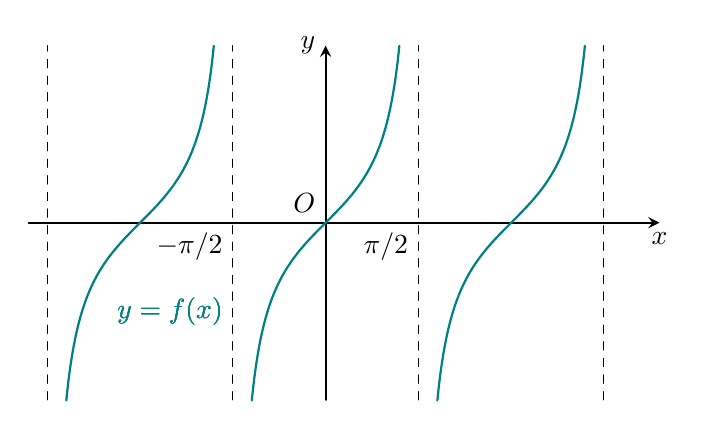
\begin{tikzpicture}[line join=round, line cap=round,thick,>=stealth,scale=.75 ]
	 	\draw[->](-1.6*pi,0)--(1.8*pi,0) node[below]{$x$};
	 	\draw[->](0,-3)--(0,3) node[left]{$y$};
	 	\draw (0,0) node[above left]{$O$};
	 	\foreach \i in {-1,0,1}{
	 		\pgfmathsetmacro{\start}{\i*pi-1.25}
	 		\pgfmathsetmacro{\left}{(\i-0.5)*pi}
	 		\pgfmathsetmacro{\end}{\i*pi+1.25}
	 		\draw[dashed, thin](\left,-3)--(\left,3);
	 		\draw[domain=\start:\end,samples=100,smooth,teal] plot(\x,{tan(\x r)}) (-3.7,-1.5) node[right]{$y=f(x)$};
	 	}
	 	\draw[dashed,thin] (1.5*pi,-3)--(1.5*pi,3);
	 	\draw (-pi/2,0) node [below left]{$-\pi/2$} (pi/2,0) node [below left]{$\pi/2$};
	 \end{tikzpicture}	
	 }
	\loigiai
	{
		Quan sát đồ thị hàm số, ta có	
		\begin{itemize}
			\item Đồ thị hàm số là các đường liền nét trên khoảng $(-\dfrac{\pi}{2};0)$, $(0;\dfrac{\pi}{2}) $ do đó hàm số liên tục trên các khoảng này.
			\item Hàm số $y=f(x)$ gián đoạn tại các điểm $x_0=\dfrac{\pi}{2}$ và $x_0=-\dfrac{\pi}{2}$.
		\end{itemize}
	}
\end{ex}
 
\Closesolutionfile{ans}

